\documentclass[11pt,a4paper]{article}
\usepackage[a4paper,margin=2.4cm]{geometry}
\usepackage[T1]{fontenc}
\usepackage[french]{babel}
\usepackage{lmodern}
\usepackage{graphicx,xcolor,booktabs,array,tabularx}
\usepackage{amsmath}
\usepackage{tikz}
\usetikzlibrary{positioning,arrows.meta,fit,calc}
\usepackage{enumitem,caption,fancyhdr,lastpage,microtype}

\definecolor{accent}{HTML}{8B1E2D}
\definecolor{grisfond}{HTML}{F5F5F7}
\definecolor{grisligne}{HTML}{D6D8DE}
\definecolor{gristexte}{HTML}{5B616B}
\usepackage[colorlinks=true,linkcolor=accent,urlcolor=accent,citecolor=accent]{hyperref}

\captionsetup{font=small,labelfont={bf,color=accent}}
\setlist[itemize]{leftmargin=1.3em,itemsep=2pt,topsep=3pt,parsep=0pt}
\setlist[enumerate]{leftmargin=1.5em,itemsep=2pt,topsep=3pt,parsep=0pt}
\setlength{\parskip}{4pt}
\setlength{\parindent}{0pt}
\emergencystretch=2em
\hbadness=5000

\newcommand{\code}[1]{\texttt{\detokenize{#1}}}

\pagestyle{fancy}\fancyhf{}
\renewcommand{\headrulewidth}{0.4pt}
\fancyhead[L]{\small\textcolor{gristexte}{MedievAIl Battle P2P}}
\fancyhead[R]{\small\textcolor{gristexte}{Rapport technique}}
\fancyfoot[C]{\small\thepage\ / \pageref{LastPage}}

\begin{document}

%================================================================ TITRE
\begin{center}
{\Huge\bfseries\color{accent} MedievAIl Battle P2P}\\[6pt]
{\Large Infrastructure r\'eseau pair-\`a-pair pour IA distribu\'ees\\[2pt] daemon en C, jeu en Python, synchronisation par UDP}\\[10pt]
{\large Rapport technique}\\[10pt]
{\small Projet collectif STI3A (projet r\'eseaux) --- INSA Centre-Val de Loire --- octobre 2025 \`a avril 2026\\
Rapport r\'edig\'e en octobre 2026 \`a partir du d\'ep\^ot, par Mohamed Aziz BAOUEB (\href{https://github.com/aziz3r}{@aziz3r}), mainteneur du miroir\\[2pt]
Code source : \url{https://github.com/aziz3r/medievail-battle-p2p}}
\end{center}
\vspace{-2pt}
\noindent\rule{\linewidth}{0.8pt}

\begin{abstract}\noindent
MedievAIl Battle P2P prolonge le jeu de bataille m\'edi\'eval d\'evelopp\'e pour le projet Python de la formation : deux joueurs, chacun avec son
arm\'ee et son IA, s'affrontent sans serveur central. Chaque machine ex\'ecute deux processus : le jeu (Python, pygame) et un daemon r\'eseau
\'ecrit en C qui relaie les messages en UDP vers le pair. Ce rapport d\'ecrit l'architecture, le protocole de lobby et de synchronisation,
l'historique du d\'eveloppement, puis une exp\'erience r\'ealis\'ee en octobre 2026 : une partie compl\`ete entre deux instances locales, enregistr\'ee
c\^ote \`a c\^ote. L'exp\'erience montre un fonctionnement de bout en bout (lobby, placement, combat) mais aussi une divergence des deux vues en fin de
bataille, et r\'ev\`ele une limite propre \`a macOS : le daemon d'origine perd les paquets de plus de 9\,Ko. Le rapport confronte enfin la
documentation au code et propose des pistes d'am\'elioration. Le projet est une \oe uvre collective ; l'historique Git d'origine est conserv\'e.
\end{abstract}

\setcounter{tocdepth}{1}
\tableofcontents

%================================================================ 1
\section{Contexte et objectifs}

Ce d\'ep\^ot est un miroir, maintenu par \href{https://github.com/aziz3r}{@aziz3r}, du projet r\'eseaux de la formation STI3A de l'INSA Centre-Val de Loire
(d\'ep\^ot de r\'ef\'erence : \href{https://github.com/YOUSSEF4315/STI3A-Projet_reseaux_1}{YOUSSEF4315/STI3A-Projet\_reseaux\_1} ; voir \code{AUTHORS.md}
pour les onze contributeurs et leurs droits). Il repose sur la base de jeu du projet Python / POO, d\'ecrite dans le d\'ep\^ot
\href{https://github.com/aziz3r/medievail-battle}{medievail-battle} : les deux historiques sont communs jusqu'au 27 janvier 2026. Le code r\'eseau est l'apport
de ce d\'ep\^ot ; il a \'et\'e \'ecrit entre le 8 et le 29 avril 2026 (21 commits) et le d\'ep\^ot compte 132 commits d'\'equipe au total.

L'objectif, tel que l'\'enonce le README, est de fournir une \emph{infrastructure r\'eseau d\'ecentralis\'ee} pour un jeu de bataille strat\'egique, avec
une s\'eparation stricte des responsabilit\'es : la logique de jeu, les IA et l'interface restent dans le processus Python ; la communication entre pairs
est confi\'ee \`a un processus C. L'int\'er\^et p\'edagogique est de manipuler sockets UDP, communication inter-processus (IPC), coh\'erence d'un \'etat partag\'e
sans serveur et d\'efauts typiques des r\'eseaux non fiables.

Les chiffres cit\'es sans r\'ef\'erence ont \'et\'e mesur\'es en octobre 2026 sur un Mac (Python 3.9.6, pygame 2.6.1, compilateur de macOS) ; ils sont indicatifs.
Le code compte environ 6\,500 lignes de Python (1\,972 pour le mod\`ele, 2\,134 pour la vue, 1\,616 pour le pr\'esentateur et 762 \`a la racine) et 177 lignes de C.

%================================================================ 2
\section{Architecture}

\begin{figure}[h]\centering
\begin{tikzpicture}[font=\scriptsize,>={Stealth},
  boite/.style={draw=grisligne,fill=grisfond,rounded corners=3pt,inner sep=5pt,align=center,minimum width=3.8cm,minimum height=1.1cm},
  machine/.style={draw=accent,rounded corners=4pt,inner sep=9pt,dashed}]
\node[boite] (py1) {Jeu Python\\[1pt]IA, interface, \'etat de la partie};
\node[boite,below=16mm of py1] (c1) {Daemon r\'eseau C\\[1pt]\texttt{reseau.c}};
\node[boite,right=40mm of py1] (py2) {Jeu Python\\[1pt]IA, interface, \'etat de la partie};
\node[boite,below=16mm of py2] (c2) {Daemon r\'eseau C\\[1pt]\texttt{reseau.c}};
\node[machine,fit=(py1)(c1),label={[font=\scriptsize\bfseries,text=accent]above:Machine du joueur 1 (h\^ote)}] {};
\node[machine,fit=(py2)(c2),label={[font=\scriptsize\bfseries,text=accent]above:Machine du joueur 2 (client)}] {};
\draw[<->,thick] (py1) -- node[right,font=\tiny,align=left]{IPC UDP local\\5000 / 5001} (c1);
\draw[<->,thick] (py2) -- node[right,font=\tiny,align=left]{IPC UDP local\\5002 / 5003} (c2);
\draw[<->,thick,color=accent] (c1) -- node[above,font=\tiny]{UDP pair-\`a-pair} node[below,font=\tiny]{6000 $\leftrightarrow$ 6001} (c2);
\end{tikzpicture}
\caption{Topologie : chaque joueur ex\'ecute deux processus. Le jeu ne parle qu'\`a son daemon local ; seuls les daemons C communiquent \`a travers le r\'eseau.
Les num\'eros sont ceux du README (test sur une seule machine).}
\end{figure}

\subsection{Le daemon r\'eseau (\code{reseau.c})}

Le daemon est un relais UDP \`a une seule boucle \code{select()}. Il se lance avec cinq param\`etres
(\code{reseau <port_p2p_local> <ip_distante> <port_p2p_distant> <ipc_entrant> <ipc_sortant>}) et surveille deux sockets : un socket local
(\code{127.0.0.1}, port IPC entrant) et un socket r\'eseau (\code{0.0.0.0}, port P2P). Le comportement est le suivant :
\begin{itemize}
  \item \emph{jeu $\to$ r\'eseau} : tout datagramme re\c cu sur le port IPC entrant est transmis tel quel au pair, et le daemon renvoie un accus\'e local (\code{{"type": "ack"}}) ;
  \item \emph{r\'eseau $\to$ jeu} : tout datagramme re\c cu sur le port P2P est renvoy\'e au jeu local, sur le port IPC sortant ;
  \item l'adresse du pair est mise \`a jour avec l'adresse source du dernier paquet re\c cu (IP et port), ce qui permet de d\'ecouvrir le pair dynamiquement.
\end{itemize}
Le tampon de lecture est de 64\,Ko. Le code est portable (Winsock sous Windows, sockets POSIX ailleurs).

\subsection{Le pont Python (\code{network_ipc.py})}

La classe \code{IPCClient} ouvre deux sockets UDP : un pour envoyer au daemon (port IPC entrant) et un, non bloquant, pour recevoir sur le port IPC sortant.
Les messages sont des dictionnaires s\'erialis\'es en JSON ; \code{receive()} lit au plus un datagramme par appel, sans jamais bloquer le jeu. Les tampons
d'envoi et de r\'eception sont port\'es \`a 65\,535 octets. Un routeur de secours en Python (\code{p2p_node_mock.py}), de m\^eme interface, remplace le daemon C
quand aucun compilateur n'est disponible ; c'est lui qui sert pour la \og version 1 \fg{} du README.

\subsection{Ports}

\begin{table}[h]\centering\small
\begin{tabular}{@{}lrrrr@{}}
\toprule
Joueur & Port P2P (daemon) & Port du pair & IPC entrant & IPC sortant \\
\midrule
Joueur 1 (h\^ote) & 6000 & 6001 & 5000 & 5001 \\
Joueur 2 (client) & 6001 & 6000 & 5002 & 5003 \\
\bottomrule
\end{tabular}
\caption{Configuration pour tester les deux joueurs sur une m\^eme machine (les ports IPC diff\`erent pour \'eviter tout conflit).}
\end{table}

%================================================================ 3
\section{Protocole et d\'eroulement d'une partie}

\subsection{Lobby}

Depuis le menu, \og Multijoueur (P2P) \fg{} ouvre un lobby : chaque joueur choisit son IA et l'une des quatre zones de d\'eploiement (quadrants de la carte
120$\times$120), puis cr\'ee la partie (h\^ote) ou la rejoint (client). Le jeu envoie alors toutes les 0,5 seconde un message de choix et attend celui de l'adversaire,
pendant 10 secondes au plus :
\begin{verbatim}
{"type": "setup_choice", "ia": "General STRATEGUS", "zone": 1}
\end{verbatim}
Chaque processus cr\'ee ensuite \emph{localement} les deux arm\'ees : 150 unit\'es par camp (50 piquiers, 50 chevaliers, 50 arbal\'etriers, sur deux colonnes de 25 lignes
chacun), plac\'ees dans le quadrant choisi. L'\'equipe locale est \code{A} pour l'h\^ote et \code{B} pour le client, et chaque unit\'e re\c coit un identifiant stable
\code{A_1}, \code{A_2}, \ldots{} Seule l'IA locale est instanci\'ee : l'adversaire est pilot\'e \`a distance.

\begin{table}[h]\centering\small
\begin{tabular}{@{}lcc@{}}
\toprule
Zone & $x$ & $y$ \\
\midrule
1 (haut-gauche) & 10--50 & 10--50 \\
2 (haut-droite) & 70--110 & 10--50 \\
3 (bas-gauche) & 10--50 & 70--110 \\
4 (bas-droite) & 70--110 & 70--110 \\
\bottomrule
\end{tabular}
\caption{Quadrants de d\'eploiement (\code{QUADRANT_BOUNDS} dans \code{model/army_compositions.py}).}
\end{table}

\subsection{Placement et d\'emarrage}

La partie s'ouvre en phase de \emph{placement} : le jeu ne simule rien (pas de temps \code{dt=0}) mais continue de recevoir l'\'etat du pair ; un clic gauche ajoute
un chevalier \`a l'arm\'ee locale. La touche \texttt{ENTR\'EE} d\'emarre le combat \emph{pour le joueur local seulement} : aucun message n'est \'echang\'e pour d\'emarrer
les deux simulations ensemble.

\subsection{Synchronisation de l'\'etat}

Pendant la partie, chaque instance appelle \code{Game.step} \`a chaque image. Au d\'ebut du pas, elle lit au plus un datagramme du daemon et l'applique ; \`a la fin
du pas, une fois sur cinq, elle diffuse son \'etat compact (exemple de contenu) :
\begin{verbatim}
{"t": "as", "u": {"A_1": {"tp": "Pikeman", "x": 31.0, "y": 17.0, "h": 55.0},
                  "B_1": {"h": 55.0}, ...}}
\end{verbatim}
Pour chaque unit\'e de l'\'equipe locale (le \og propri\'etaire \fg{}), le message contient le type, la position et les points de vie ; pour les unit\'es de
l'adversaire, uniquement les points de vie, afin de propager les d\'egats inflig\'es. \`A la r\'eception, les positions ne sont appliqu\'ees qu'aux unit\'es de l'autre \'equipe
(l'IA locale reste ma\^itresse des siennes), les unit\'es inconnues sont cr\'e\'ees, et les points de vie re\c cus sont \'ecrits sur toutes les unit\'es.

\textbf{Taille des paquets.} Avec 150 unit\'es par camp, un message complet p\`ese 12\,502 octets au d\'epart, soit 42 octets par unit\'e. \`A 30 images par seconde,
un paquet toutes les 5 images repr\'esente 6 paquets par seconde, environ 75\,Ko/s dans chaque sens (estimation). Comme la taille cro\^it lin\'eairement avec
l'effectif et qu'un datagramme UDP ne peut pas d\'epasser 65\,507 octets, ce sch\'ema est born\'e \`a environ 1\,500 unit\'es en tout.

%================================================================ 4
\section{Historique du d\'eveloppement}

L'historique Git permet de suivre la construction de la partie r\'eseau :

\begin{table}[h]\centering\small
\begin{tabularx}{\linewidth}{@{}l l X@{}}
\toprule
Date & Auteur (Git) & Contenu \\
\midrule
8 avril 2026 & zaydbouazza & Champs r\'eseau de \code{Guerrier} : identifiant, propri\'etaire, s\'erialisation. \\
9 avril & zaydbouazza & Couche r\'eseau UDP + IPC entre C et Python. \\
10 avril & Ali ; aziz3r & Int\'egration de la synchronisation dans \code{Game} ; lobby multijoueur (IA et zone), corrections de plantages de synchro, UID stables, scripts de test et preuve de concept. \\
28 avril & Ali, YOUSSEF4315, zaydbouazza & README ; routeur de secours en Python ; simulation de perte de paquets ajout\'ee puis retir\'ee ; correction de doublons d'unit\'es ; \og finalisation V1 \fg{} (tampons maximaux, grandes arm\'ees). \\
29 avril & Ali, YOUSSEF4315 & Arm\'ees de 520 puis de 150 unit\'es par \'equipe ; bug visuel \og mort-vivant \fg{} pour la pr\'esentation ; README V1/V2 et sch\'emas. \\
\bottomrule
\end{tabularx}
\caption{Chronologie du code r\'eseau, d'apr\`es les messages de commits (les noms sont ceux qui figurent dans l'historique).}
\end{table}

Le README distingue deux versions. La \textbf{version 1} est une couche r\'eseau \og best-effort \fg{} : les actions sont diffus\'ees sans garantie de r\'eception ni d'ordre, ce qui
produit des unit\'es dupliqu\'ees, des \og fant\^omes \fg{} et des d\'esynchronisations (routeur Python, utilis\'e pour montrer les d\'efauts d'un r\'eseau sans protocole de coh\'erence). La \textbf{version 2} annonce un
daemon C avec une notion de \emph{propri\'et\'e r\'eseau} (une seule entit\'e propri\'etaire \`a un instant donn\'e, n\'egociation du transfert avec les pairs), des m\'ecanismes anti-zombie et
une victoire synchronis\'ee. La section~\ref{sec:analyse} compare cette description au code pr\'esent dans le d\'ep\^ot.

%================================================================ 5
\section{Exp\'erience : une partie compl\`ete entre deux instances locales}

\subsection{Protocole d'exp\'erience}

Nous avons ex\'ecut\'e le v\'eritable jeu et le v\'eritable daemon sur une m\^eme machine : deux daemons (ports du tableau~1), deux instances du jeu pilot\'ees par un script
(souris et clavier simul\'es, affichage sans fen\^etre, temps virtuel \`a 30 images/s), enregistr\'ees c\^ote \`a c\^ote. Le joueur 1 (h\^ote) joue General STRATEGUS en zone 1,
le joueur 2 (client) joue Major DAFT en zone 4. Le script et les m\'edias sont dans \code{demo/} ; il se relance avec \code{python demo/capture_demo.py}.

\begin{figure}[h]\centering
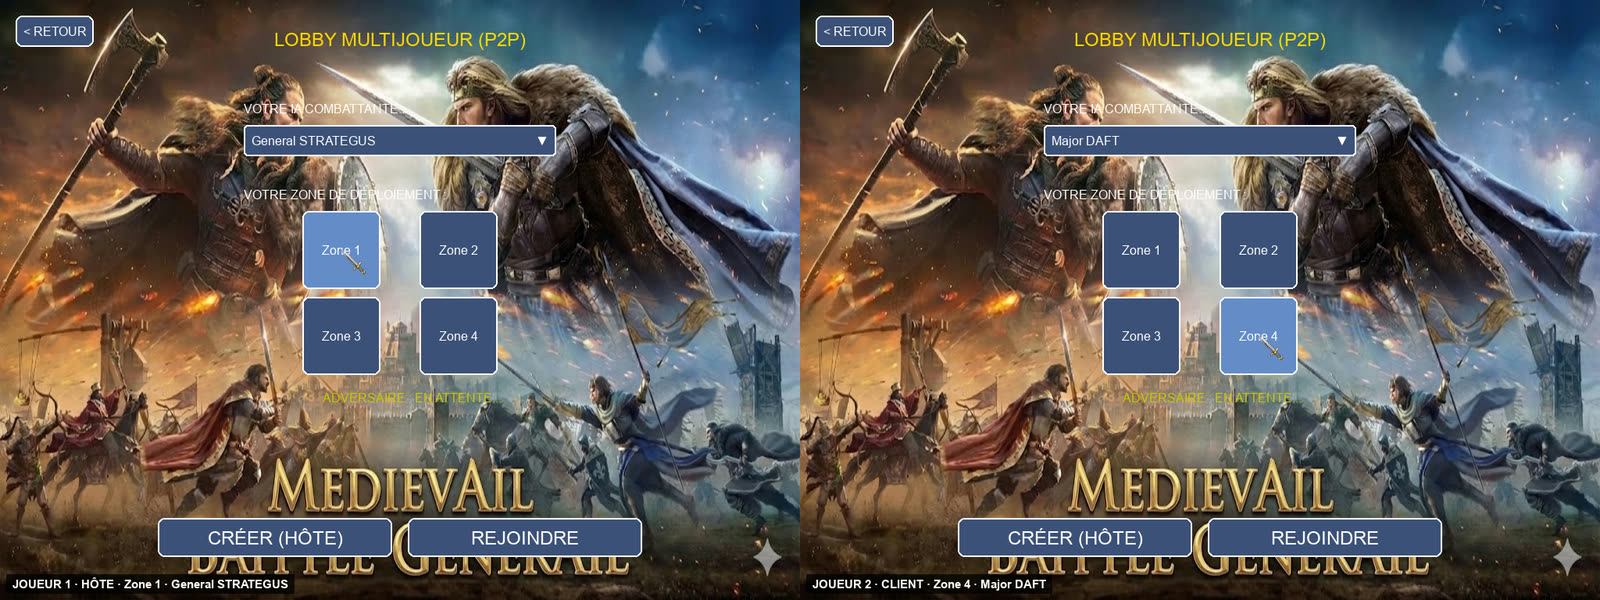
\includegraphics[width=\linewidth]{figures/03_lobby_pret.jpg}
\caption{Lobby des deux joueurs apr\`es le choix de l'IA et de la zone (h\^ote \`a gauche, client \`a droite).}
\end{figure}

\subsection{Observations}

\textbf{Le trafic passe bien par les daemons C.} Sur la partie enregistr\'ee, le daemon de l'h\^ote a transmis 662 paquets au pair et celui du client 384, ce qui est coh\'erent avec
un paquet toutes les 5 images. Le lobby, le placement des deux arm\'ees et le d\'ebut du combat se d\'eroulent comme d\'ecrit : les deux \'ecrans montrent les m\^emes arm\'ees et chaque
joueur voit bouger les unit\'es de l'adversaire (figure~\ref{fig:melee}).

\begin{figure}[h]\centering
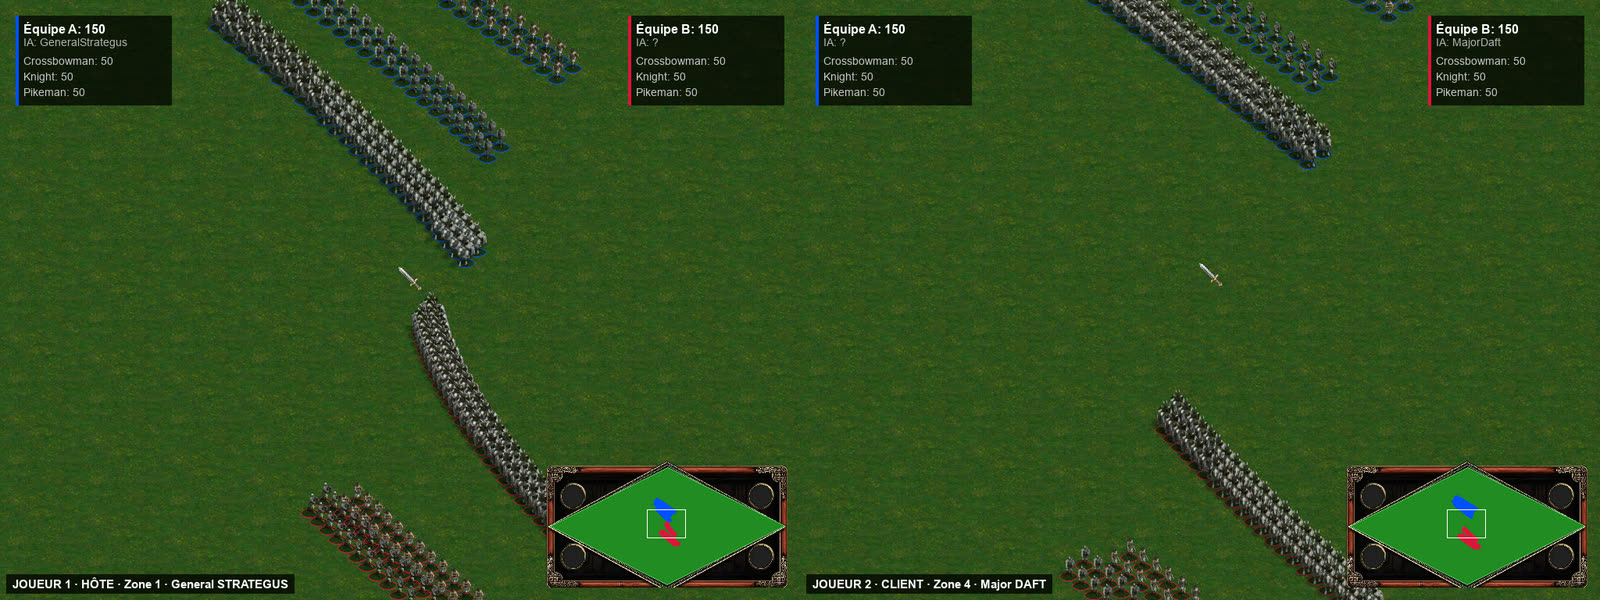
\includegraphics[width=\linewidth]{figures/06_melee.jpg}
\caption{\label{fig:melee}Les deux arm\'ees avancent l'une vers l'autre (m\^eme instant du script ; h\^ote \`a gauche, client \`a droite).}
\end{figure}

\textbf{Les deux vues finissent par diverger.} \`A la fin de l'enregistrement, le client affiche \og Victoire \'equipe B \fg{} (\'equipe A : 0 unit\'e, \'equipe B : 112), alors que l'h\^ote affiche encore
\'equipe A : 1 et \'equipe B : 108 et n'a pas d\'etect\'e de fin de partie. Des unit\'es teint\'ees en vert --- le drapeau \code{is_zombie}, voir la section~\ref{sec:analyse} --- apparaissent pendant la m\^el\'ee.
L'h\^ote a d'ailleurs jou\'e plus longtemps que le client (117 s contre 77 s enregistr\'ees).

\begin{figure}[h]\centering
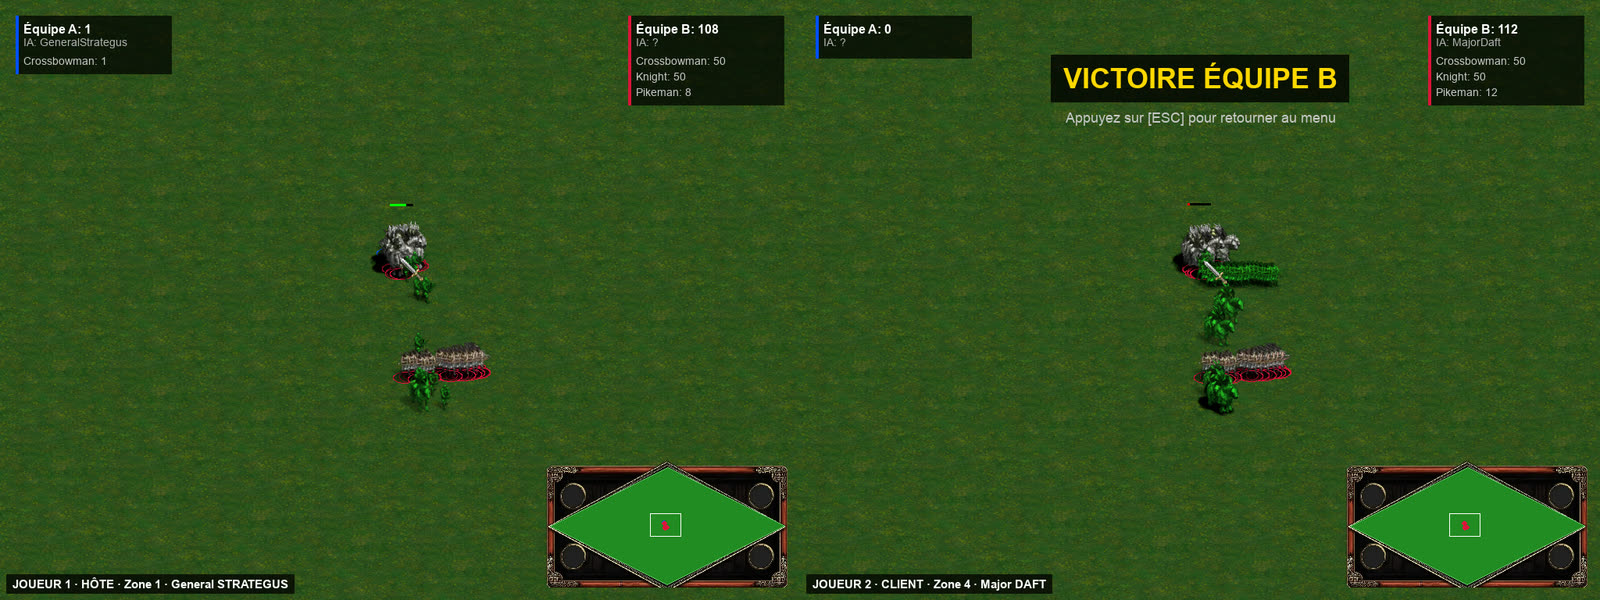
\includegraphics[width=\linewidth]{figures/08_fin_de_bataille.jpg}
\caption{\'Etat final affich\'e par chaque joueur. Les deux captures sont prises \`a la fin du script de chaque joueur, donc pas au m\^eme instant.}
\end{figure}

Ces observations proviennent d'une seule ex\'ecution. Le script de capture rend les images \`a des vitesses qui diff\`erent d'un joueur \`a l'autre (rendu sans fen\^etre) alors
que la synchronisation d\'epend du rythme des images : cela peut avoir amplifi\'e la divergence, sans que nous puissions la quantifier.

\subsection{Un obstacle propre \`a macOS : la taille maximale d'un datagramme}

Sous macOS, la taille maximale d'un datagramme UDP est limit\'ee par d\'efaut \`a 9\,216 octets (\code{sysctl net.inet.udp.maxdgram}), et \code{reseau.c} ne r\`egle pas la taille des tampons
de ses sockets (\code{SO_SNDBUF}). Nous avons envoy\'e au daemon des datagrammes de tailles croissantes depuis \code{network_ipc.py} et v\'erifi\'e leur arriv\'ee au pair :

\begin{table}[h]\centering\small
\begin{tabular}{@{}rl@{}}
\toprule
Taille du message & Re\c cu par le jeu du pair (daemon d'origine) \\
\midrule
1\,000 octets & oui \\
8\,000 octets & oui \\
12\,000 octets & \textbf{non} (perdu) \\
30\,000 octets & \textbf{non} (perdu) \\
\bottomrule
\end{tabular}
\caption{Test du daemon d'origine compil\'e sur macOS (une exp\'erience par taille).}
\end{table}

Or le premier message de synchronisation fait 12\,502 octets : avec le daemon d'origine, la synchronisation du combat ne peut pas passer sur ce syst\`eme.
Pour la d\'emonstration, le script compile donc une \emph{copie temporaire} de \code{reseau.c} dans laquelle les tampons des deux sockets sont port\'es \`a 1\,Mo ; le fichier du d\'ep\^ot n'est pas modifi\'e.
Sous Linux et Windows, la limite par d\'efaut est plus large et le probl\`eme ne se pose pas dans les m\^emes termes (non test\'e).

%================================================================ 6
\section{Analyse : documentation et code\label{sec:analyse}}

\subsection{La propri\'et\'e r\'eseau annonc\'ee n'est pas dans le code}

Dans les fichiers du d\'ep\^ot :
\begin{itemize}
  \item \code{reseau.c} est un relais : il ne contient ni table de propri\'et\'e, ni consensus, ni n\'egociation de transfert ;
  \item le champ \code{proprietaire_reseau} est d\'efini et s\'erialis\'e par \code{Guerrier.to_dict} / \code{update_from_dict}, mais ces deux m\'ethodes ne sont jamais appel\'ees ;
  \item la synchronisation r\'eelle passe par \code{get_sync_state} / \code{apply_sync_state}, qui \'ecrit sans arbitrage les points de vie re\c cus sur n'importe quelle unit\'e. Un commentaire annonce
        \og on prend le minimum pour ne jamais annuler un d\'egat subi \fg{}, mais le code qui suit \'ecrit la valeur re\c cue, et un second commentaire parle de \og cr\'eation du bug de rollback \fg{}.
\end{itemize}

\textbf{M\'ecanisme du zombie.} Chaque pair diffuse les points de vie de \emph{toutes} les unit\'es qu'il conna\^it, y compris celles de l'adversaire. Si le pair a une valeur p\'erim\'ee, elle \'ecrase la valeur \`a jour
de l'unit\'e propri\'etaire : l'unit\'e retrouve des points de vie perdus (rollback), ou \emph{ressuscite} si elle \'etait morte. Le code l'assume : lorsqu'une unit\'e morte localement re\c coit des points de vie positifs,
elle est marqu\'ee \code{is_zombie} et dessin\'ee en vert. Le commit du 29 avril intitul\'e \og Visual Zombie bug (Mort-Vivant) implementation for presentation \fg{} sugg\`ere que ce comportement a \'et\'e ajout\'e
volontairement, pour illustrer le probl\`eme lors de la pr\'esentation. Le d\'ep\^ot est donc coh\'erent avec ce que nous observons ; en revanche, les m\'ecanismes de la version 2 (propri\'et\'e, anti-zombie, victoire synchronis\'ee) d\'ecrits dans le README
ne sont pas impl\'ement\'es dans les fichiers pr\'esents.

\subsection{Autres limites rep\'er\'ees}

\begin{itemize}
  \item \textbf{UDP sans fiabilit\'e applicative.} Pas de num\'ero de s\'equence, d'horodatage ni de d\'etection de doublons : chaque paquet contient un \'etat complet, ce qui tol\`ere la perte mais pas le d\'esordre ni
        les valeurs p\'erim\'ees.
  \item \textbf{D\'emarrage et fin non synchronis\'es.} \texttt{ENTR\'EE} d\'emarre la simulation du seul joueur local, et chaque pair calcule la victoire sur son propre \'etat ; aucun message de d\'ebut ou de fin n'existe.
  \item \textbf{Une seule lecture par pas.} Le jeu ne lit qu'un datagramme par image ; ce n'est pas bloquant au d\'ebit actuel, mais le d\'ebit de r\'eception n'est pas contr\^ol\'e.
  \item \textbf{Taille born\'ee.} Voir la section~3.3 : le message cro\^it avec l'effectif et d\'epasse la limite par d\'efaut de macOS \`a environ 220 unit\'es.
  \item \textbf{S\'ecurit\'e.} Aucune authentification ni chiffrement ; le daemon \'ecoute sur toutes les interfaces et adopte comme pair l'exp\'editeur du dernier paquet re\c cu ; plusieurs erreurs de r\'eseau sont
        ignor\'ees (blocs \code{except} qui se terminent par \code{pass}). \`A ne pas exposer en dehors d'un r\'eseau de confiance.
  \item \textbf{Scripts de test.} \code{verify_sync.py} lance deux daemons avec les ports IPC par d\'efaut, identiques : le second quitte avec l'erreur \code{bind(): Address already in use} (v\'erifi\'e). Il appelle aussi \code{./reseau}
        alors que le README compile \code{reseau.exe}, et g\'en\`ere \code{test_joiner.py} \`a la vol\'ee.
  \item \textbf{Fichiers parasites.} Un ex\'ecutable compil\'e (\code{network_poc/p2p_node}, binaire macOS arm64 de 34\,Ko) et une copie temporaire encod\'ee en UTF-16 (\code{temp_remote_network_ipc.py}) sont versionn\'es.
  \item \textbf{Documentation de compilation.} Le README donne la commande Windows (\code{-lws2_32}) ; sous macOS, \code{gcc reseau.c -o reseau -lpthread} suffit (la limite des datagrammes mentionn\'ee plus haut s'applique).
\end{itemize}

%================================================================ 7
\section{Reproductibilit\'e}

Pour rejouer l'exp\'erience du README sur une machine (quatre terminaux), avec la version 2 :
\vspace{3pt}\noindent\begin{minipage}{\linewidth}\small
\begin{verbatim}
gcc reseau.c -o reseau -lpthread          # Linux / macOS
./reseau 6000 127.0.0.1 6001 5000 5001    # terminal 1 : daemon hote
python launch.py                          # terminal 2 : menu 6, zone 1, CREER
./reseau 6001 127.0.0.1 6000 5002 5003    # terminal 3 : daemon client
python launch.py                          # terminal 4 : menu 6, zone 4, REJOINDRE
\end{verbatim}
\end{minipage}\vspace{5pt}
Sous macOS, les messages de synchronisation de 150 unit\'es par camp d\'epassent la taille maximale d'un datagramme (section~5.3) ; la d\'emonstration automatis\'ee
(\code{python demo/capture_demo.py}) contourne ce point avec une copie temporaire du daemon.

%================================================================ 8
\section{Pistes d'am\'elioration}

\begin{enumerate}
  \item Impl\'ementer l'arbitrage annonc\'e : propri\'etaire unique de chaque unit\'e, d\'egats transmis comme \'ev\'enements (ou valeur minimale des points de vie) au lieu d'\'etats \'ecrits aveugl\'ement.
  \item Ajouter num\'eros de s\'equence et horodatage aux messages pour ignorer les paquets p\'erim\'es ou dupliqu\'es.
  \item Ajouter un message de d\'epart (\og pr\^et \fg{}, puis d\'ebut commun) et un message de fin de partie pour que les deux joueurs concluent de la m\^eme mani\`ere.
  \item R\'eduire la taille des messages (diff\'erences d'\'etat, entiers courts) ou pr\'evoir la fragmentation, et r\'egler \code{SO_SNDBUF} / \code{SO_RCVBUF} dans \code{reseau.c} pour macOS.
  \item Envisager un mod\`ele \emph{lockstep} : \'echanger seulement les ordres des IA, avec une graine d'al\'ea commune, pour rendre la simulation d\'eterministe et les messages tr\`es petits.
  \item \'Ecrire un test automatis\'e sur l'interface locale (deux \code{IPCClient}, deux relais) et corriger \code{verify_sync.py} (ports IPC distincts) ; retirer les fichiers binaires et temporaires du d\'ep\^ot.
\end{enumerate}

\end{document}
